\documentclass{article}
\usepackage{amsmath,amssymb,setspace,verbatim,graphicx,enumerate,enumitem}
\usepackage[top=1in,bottom=1in,left=1in,right=1in,head=0.5in,foot=0.5in]{geometry}
\usepackage{caption}
\usepackage{mathtools}
% \usepackage{subcaption}
% \usepackage{subfig}
% \usepackage{subfloat}
% \usepackage{tabularx}
\usepackage{mdframed}
\usepackage{amsthm}

\newtheorem*{theorem}{Theorem}

\newenvironment{Rcode}% environment name 
{%begin code
    \begin{mdframed}
    \#R code
    \begin{small}
}
{%end code
    \end{small}
    \end{mdframed}
}

\newenvironment{console}% environment name 
{%begin code
    \begin{mdframed}
    \#Console
    \begin{small}
}
{%end code
    \end{small}
    \end{mdframed}
}

\begin{document}
\title{STDA Homework 4}
\author{Seokjun Choi}
\date{June 19, 2020}
\maketitle

\textbf{Note:}
You can get full code files at my github page: Visit https://github.com/letsjdosth/SpaTempoDA \\
and see "HW4" directory. Because I provide the full code separately, in this report 
I will show key code blocks only, instead of the whole, verbose code.

\section{Problem1}
\textbf{
Alt and Vach (1991) describe an archaeological investigation of an early medieval burial ground in Germany.
One question of interest was whether grave sites tended to be place according to family units.
The data for the point process is in the file dental.reduced.dat.
Each grave has a location and an indicator variable for whether the individual had an inherited feature in the teeth or not.
}
\subsection{Case: rectangular window}
\textbf{
    (a) Load the data and create two ppp object from it, on for affected and one for unaffected individuals.
    For now, take the window to be the same for each ppp object: use a rectangular region based on the range of x and y for both datasets. \\
    (b) For each dataset separately, create Monte Carlo simulation envelopes for the F and G functions and plot them.
    Is their evidence against CSR in this dataset? If so, what type of violation is suggested?
}

In given data, the range of x-axis is $(4492, 10373)$, and of y-axis is $(3085, 10431)$ so that 
I set these range as window of ppp object.
Below is brief code of 

\begin{Rcode}
    \begin{verbatim}
library(spatstat)

dental = read.table("c:/gitProject/SpaTempoDA/Hw4/dental.reduced.dat", stringsAsFactors=FALSE)
dental.unaffected = dental[(dental[2]==0),]
dental.affected = dental[(dental[2]==1),]

rec_window = owin(xrange=c(4492, 10373), yrange=c(3085, 10431))
ppp.rec.unaffected = ppp(unlist(dental.unaffected[3]), 
                        unlist(dental.unaffected[4]), window=rec_window)
ppp.rec.affected = ppp(unlist(dental.affected[3]), 
                        unlist(dental.affected[4]), window=rec_window)
    \end{verbatim}
\end{Rcode}

In order to see the data, I report a plot of two data set.

\clearpage
\begin{figure}[!h]
    \centering
    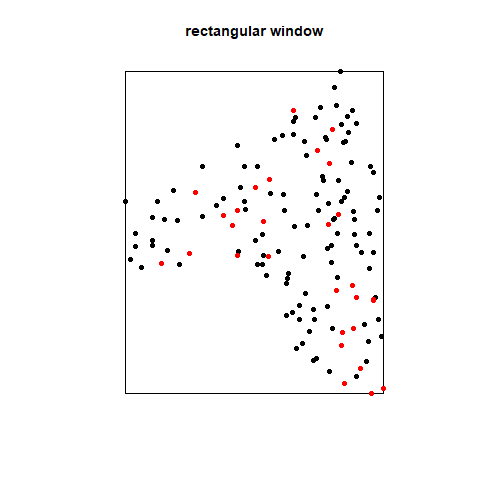
\includegraphics[width=5cm]{prob1_rectangular_window_scatterplot.png}
    \caption{scatterplot(rectangular window) : \\black: unaffected, red: affected}
\end{figure}


Next, I generate envelope to check if there are some evidences which indicate the data model against CSR or not.
Using 'envelope' function with ppp object, the code becomes quite simple. I set the number of iteration to 999 for each case.

\begin{Rcode}
    \begin{verbatim}
evlp.rec.unaffected.F = envelope(ppp.rec.unaffected, Kest, nsim = 999, nrank = 10, global = TRUE)
evlp.rec.affected.F = envelope(ppp.rec.affected, Kest, nsim = 999, nrank = 10, global = TRUE)
evlp.rec.unaffected.G = envelope(ppp.rec.unaffected, Gest, nsim = 999, nrank = 10, global = TRUE)
evlp.rec.affected.G = envelope(ppp.rec.affected, Gest, nsim = 999, nrank = 10, global = TRUE)
    \end{verbatim}
\end{Rcode}

Here are result plots.
\begin{figure}[!h]
    \centering
    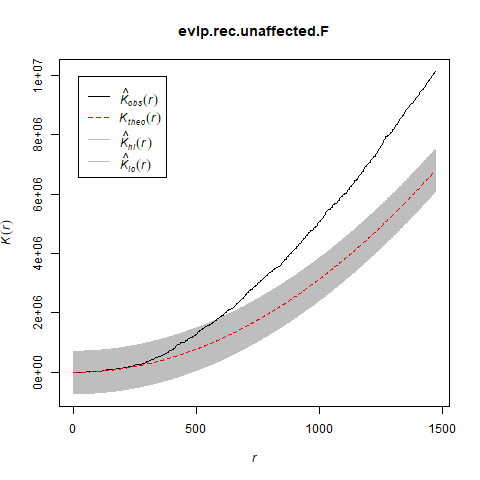
\includegraphics[width=4cm]{prob1_rectangular_window_unaffected_evlp_F.png}
    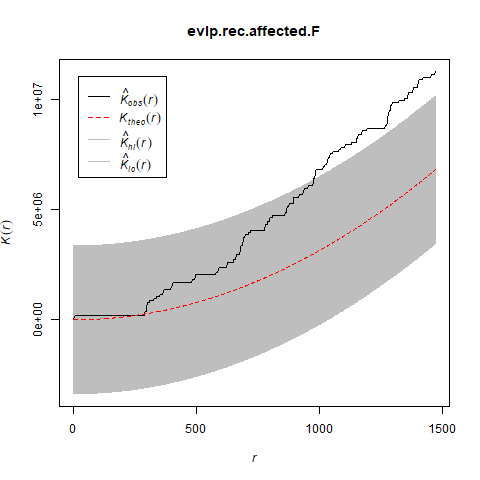
\includegraphics[width=4cm]{prob1_rectangular_window_affected_evlp_F.png} \\ 
    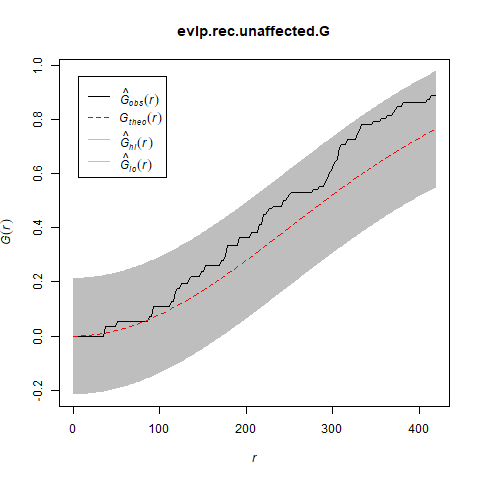
\includegraphics[width=4cm]{prob1_rectangular_window_unaffected_evlp_G.png}
    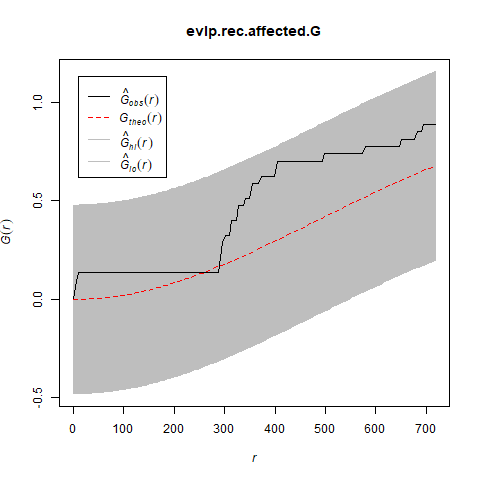
\includegraphics[width=4cm]{prob1_rectangular_window_affected_evlp_G.png}
    \caption{envelopes: \\
    upper-left: unaffected, F function, upper-right: affected, F function\\
    lower-left: unaffected, G function, lower-right: affected, G function}
\end{figure}

\clearpage
Since the estimated CDFs of using F function go out of the envelope area 
which is constructed by Monte-Carlo simulation with CSR assumption,
I get evidences which indicate the data model is not CSR.
And observe that the estimated CDF is in upper side of envelope.
It means that the data have some clustered patterns comparing to CSR.


\subsection{Case: polygon window}
\textbf{
    (c) Suppose these graves represent a complete excavation of the area in which they appear,
    and that area is irregularly shaped. Create such an outline by plotting the locations and using the locator function.
    Create two new ppp objects which this new window. \\
    (d) Repeat step (b) for the new window. What changes?
    Can you explain the reason for this, based on the form of the test statistics?
}

Run the below code block to set a polygon-shaped window and create two ppp objects.
Choose one: 
if locator\_set\_mode is TRUE, than you can set a new polygon clicking the vertices on the R-graphic device,
if locator\_set\_mode is FALSE, you can use the preset polygon.
(I proceed the preset in this report.)

\begin{Rcode}
    \begin{verbatim}
#locator
locator_set_mod = FALSE
if(locator_set_mod){
    plot(ppp.unaffected, pch = 19, main = "unaffected")
    plot(ppp.affected, pch = 19, main = "affected", col = "red", add=TRUE)
    bdry <- locator()
}else{
    #given : print(poly_window$bdry)
    bdry = list(x=c(10456.320, 9415.281, 4354.227, 4418.291,
                 5859.730, 6388.258, 8021.889, 9399.265, 10536.400),
        y=c(8333.973, 10560.196, 7677.317, 5595.238, 5579.222, 6828.470, 
                    4089.735, 3064.712, 3016.664))
}

poly_window = owin(poly=bdry)
# print(poly_window$bdry)
ppp.poly.unaffected = ppp(unlist(dental.unaffected[3]), 
                        unlist(dental.unaffected[4]), window=poly_window)
ppp.poly.affected = ppp(unlist(dental.affected[3]), 
                        unlist(dental.affected[4]), window=poly_window)
    \end{verbatim}
\end{Rcode}


In order to see the data with the new window, I also report a new plot.


\begin{figure}[!h]
    \centering
    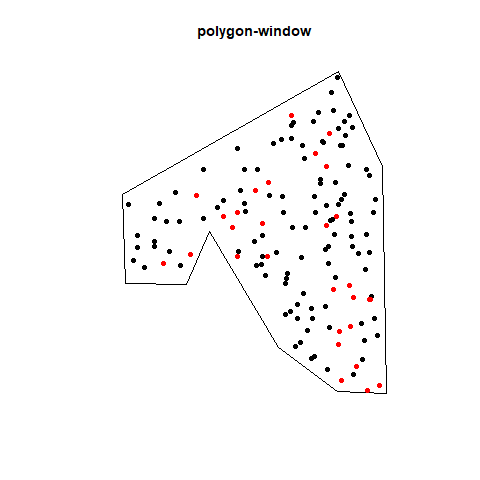
\includegraphics[width=5cm]{prob1_poly_window_scatterplot.png}
    \caption{scatterplot(polygon window) : \\black: unaffected, red: affected}
\end{figure}

Like step (a),(b), I generate envelope to check whether the data follows CSR or not.

\begin{Rcode}
    \begin{verbatim}
evlp.poly.unaffected.F = envelope(ppp.poly.unaffected, Kest, nsim = 999, nrank = 10, global = TRUE)
evlp.poly.affected.F = envelope(ppp.poly.affected, Kest, nsim = 999, nrank = 10, global = TRUE)
evlp.poly.unaffected.G = envelope(ppp.poly.unaffected, Gest, nsim = 999, nrank = 10, global = TRUE)
evlp.poly.affected.G = envelope(ppp.poly.affected, Gest, nsim = 999, nrank = 10, global = TRUE)
    \end{verbatim}
\end{Rcode}

Here are result plots.
\begin{figure}[!h]
    \centering
    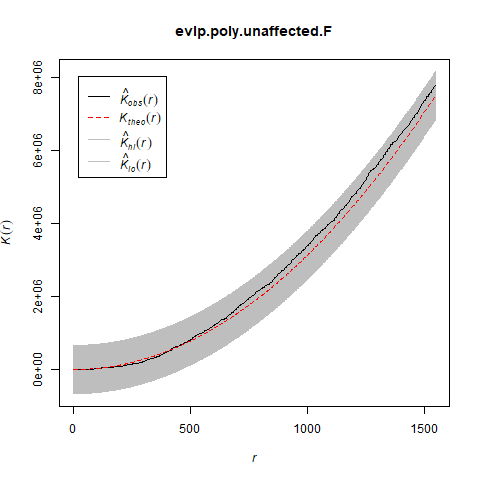
\includegraphics[width=4cm]{prob1_poly_window_unaffected_evlp_F.png}
    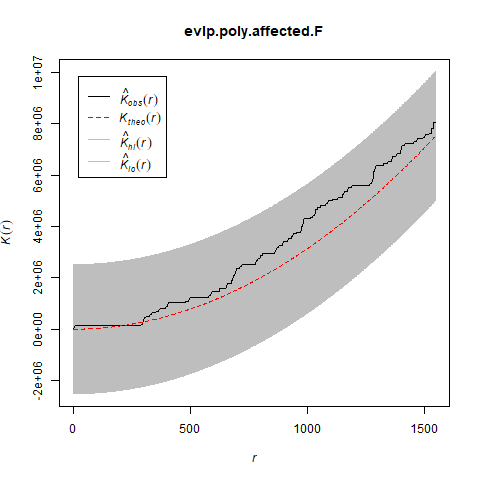
\includegraphics[width=4cm]{prob1_poly_window_affected_evlp_F.png} \\ 
    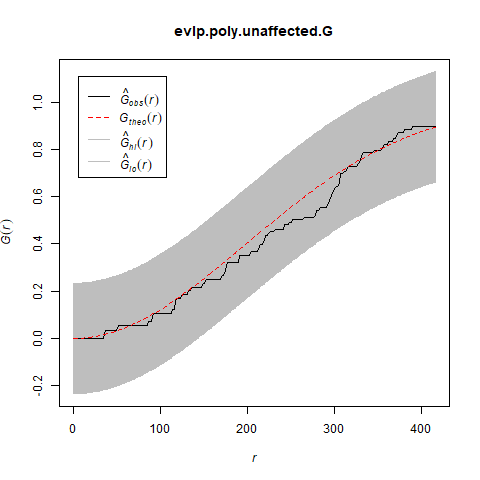
\includegraphics[width=4cm]{prob1_poly_window_unaffected_evlp_G.png}
    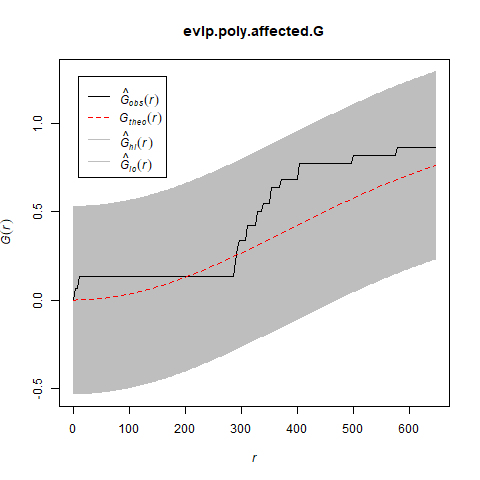
\includegraphics[width=4cm]{prob1_poly_window_affected_evlp_G.png}
    \caption{envelopes: \\
    upper-left: unaffected, F function, upper-right: affected, F function\\
    lower-left: unaffected, G function, lower-right: affected, G function}
\end{figure}

In this case, all estimated CDFs are on the envelopes constructed by MC simulation under CSR model.
So, I have no evidence that the data is against CSR.

Note that, this result is different as above rectangular window case,
especially when I use the F function for making envelopes and empirical CDFs.
This difference may be come from the property of the empty space distance
underlying F function, i.e. for a set of locations or grids $\{u_j\}_{j=1}^{N}$ at empty space,
\[\hat{F}(r) = \frac{\sum_{j=1}^{n} 1\{d(u_j, x_i)\leq x\}}{n}\]
for data point $\{x_i\}$s. 
When I use the rectangular window based on ranges of x and y,
the empty area is large, so that the grid points $\{u_j\}_{j=1}^{N}$ tend to
be located in these empty area. In contrast, when I use the polygon-shaped area,
the empty area is relatively small than the case when I use the rectangular window.
This difference yields that the values of empty space distance tend to be bigger with the rectangular window
than with the polygon-shaped window, and as a result, pushes the empirical CDFs up.
Also note that, this kind of effect is weak when I use G function which is defined with the nearest-neighbor distance,
thus the differences with G function between the case of the rectangular window and of the polygon-shaped window are smaller
than those with F function.



\clearpage
\section{Problem2}
\textbf{
Simulate four datasets on the unit square, from a homogenous Poisson process with a rate $\lambda$ of your choosing.
For each one, fit a kernel estimate of the intensity function and plot it with the points overlaid.
}

Using below R functions, I will generate four dataset on the unit square following a homogenous Poisson process.
(Two functions are basically same, but upper one shows the  procedure in detail.)

\begin{Rcode}
    \begin{verbatim}
library(spatstat)
hom_pois_process_generator = function(intensity){
    point_num = rpois(1, intensity)
    x_loc = runif(point_num,0,1)
    y_loc = runif(point_num,0,1)
    rec_window = owin(xrange=c(0, 1), yrange=c(0, 1))
    ppp.hom_pois_proc = ppp(x_loc, y_loc, window=rec_window)
    return(ppp.hom_pois_proc)
}
hom_pois_process_generator2 = function(intensity){
    rec_window = owin(xrange=c(0, 1), yrange=c(0, 1))
    return(rpoispp(intensity, lmax = 300, win = rec_window))
}
    \end{verbatim}
\end{Rcode}

I choose the intensity $\lambda=100$.
And, after generating each one, I estimate the intensity functions using kernel.
The result plots are below.

\begin{figure}[!h]
    \centering
    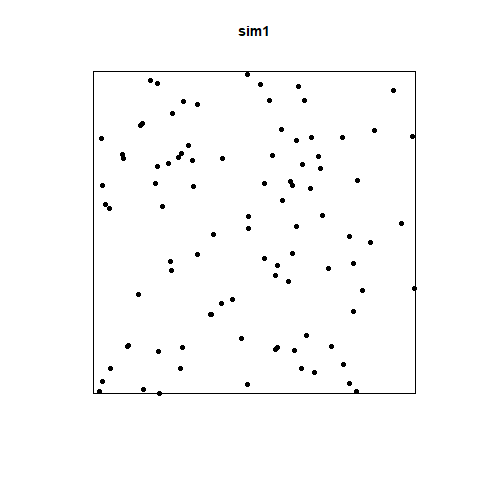
\includegraphics[width=4cm]{prob2_sim1_scatterplot.png}
    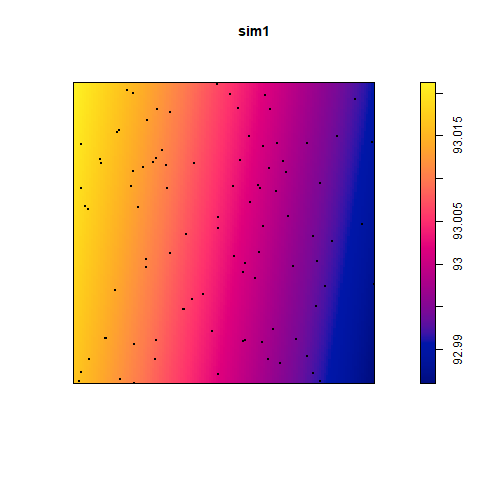
\includegraphics[width=4cm]{prob2_sim1_ker.png}
    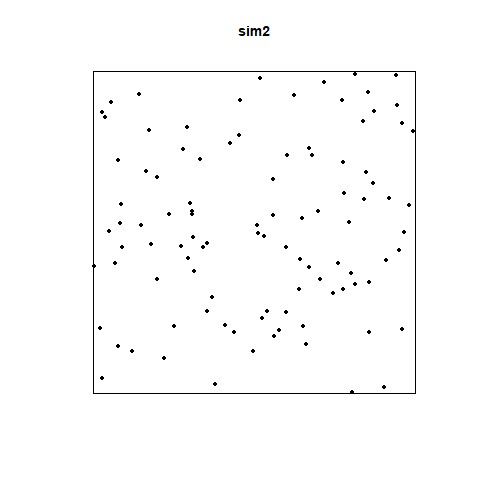
\includegraphics[width=4cm]{prob2_sim2_scatterplot.png}
    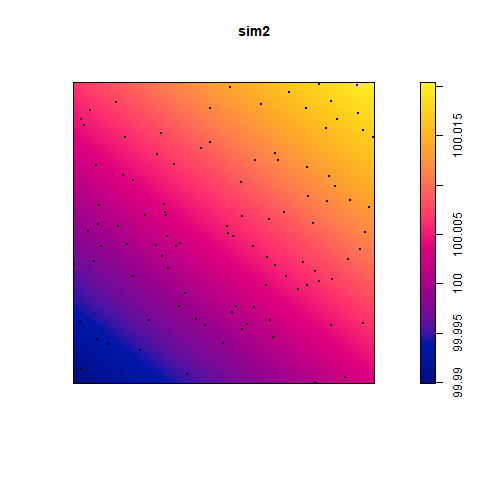
\includegraphics[width=4cm]{prob2_sim2_ker.png} \\
    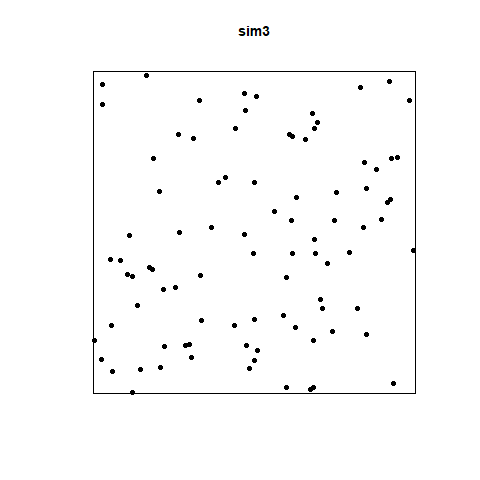
\includegraphics[width=4cm]{prob2_sim3_scatterplot.png}
    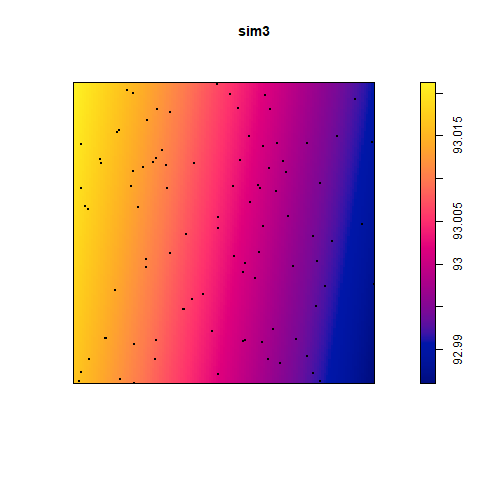
\includegraphics[width=4cm]{prob2_sim3_ker.png}
    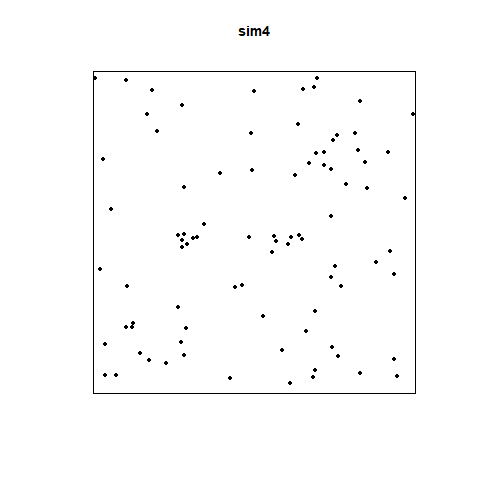
\includegraphics[width=4cm]{prob2_sim4_scatterplot.png}
    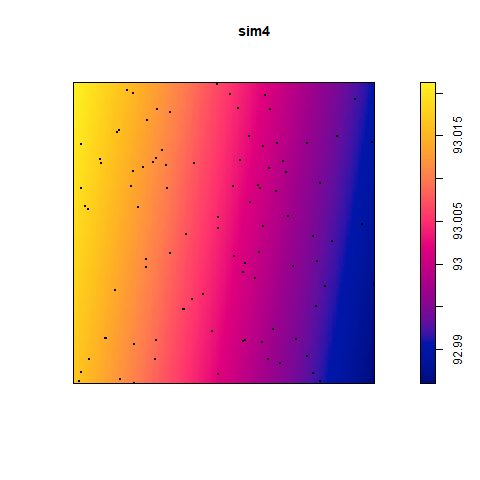
\includegraphics[width=4cm]{prob2_sim4_ker.png}
    \caption{scatterplot-estimated intensity pair: \\
    upper-left: simulation case 1, upper-right: simulation case 2, \\
    lower-left: simulation case 3, lower-right: simulation case 4}
\end{figure}

Since I use gaussian kernel to estimate the intensity functions, 
the estimated results are depend on realization of each randomly (uniformly) located points,
highest at area in which many points realized by chance, and gradually decreased as being far from the highest point.
Thus, the difference among the four estimated intensity functions are totally by chance.


\clearpage
\section{Problem3}
\textbf{
Read through section 15.2 and 15.3 of the notes by Adrian Baddeley, and
find MLEs for inhomogeneous models with intensity functions:
model 1:
\[\lambda(x) = exp(\beta_0 + \beta_1 Z(x))\]
model 2:
\[\lambda(x) = \beta Z(x)\]
Plot a kernel density estimate of $\lambda(x)$ without covariates as well as the fitted intensities under the two models.
}
In the beginning, let us see the data.
\begin{figure}[!h]
    \centering
    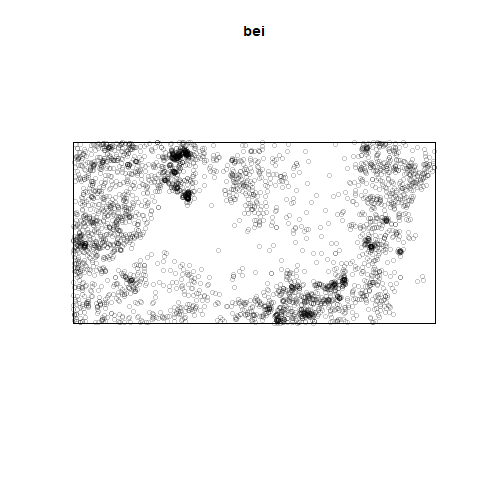
\includegraphics[width=4cm]{prob3_bei.png}
    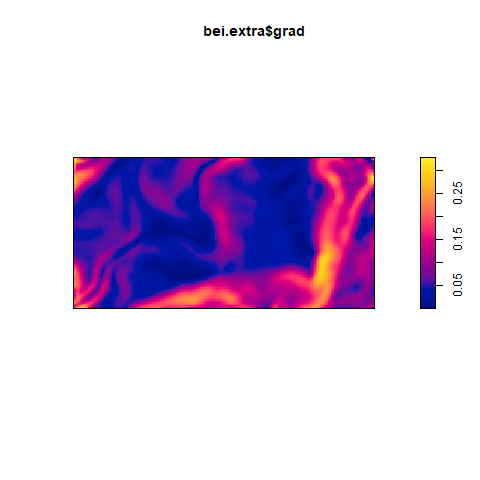
\includegraphics[width=4cm]{prob3_grad.png}
    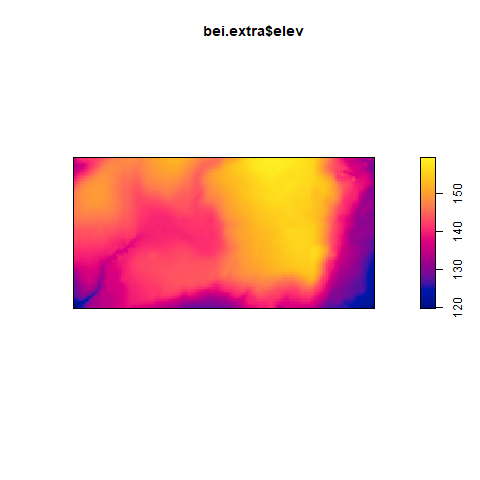
\includegraphics[width=4cm]{prob3_elev.png}
    \caption{EDA : left:bei data, middle: grad(one covariate), right: elev(another covariate)}
\end{figure}

There are one point process(in bei), and two co-variates, grad and elev(in bei.extra).
Because the given models (especially model 1) on the problem include only one variable,
hereafter, I choose the grad variable and put Z as grad data.

To fit to the models, run below code.

\begin{Rcode}
    \begin{verbatim}
library(spatstat)
data(bei)

# model 1
grad = bei.extra$grad
fit.model1 = ppm(bei, ~slope, covariates=list(slope=grad))
# model 2
fit.model2 = ppm(bei, ~offset(log(slope)), covariates = list(slope = grad))
    \end{verbatim}
\end{Rcode}

Here are summary and plots of fitting.
The values on 'Estimate' column are MLEs that we want.

Model 1:
\begin{verbatim}
                 Estimate       S.E.   CI95.lo   CI95.hi Ztest      Zval
    (Intercept) -5.391053 0.03001787 -5.449887 -5.332219   *** -179.5948
    slope        5.026710 0.24534296  4.545847  5.507573   ***   20.4885
\end{verbatim}
\[\lambda(x) = exp(-3.591053 + 5.026710 Z(x))\]

Model 2:
\begin{verbatim}
                 Estimate       S.E.   CI95.lo   CI95.hi Ztest      Zval
    (Intercept) -2.427165 0.01665742 -2.459813 -2.394517   *** -145.7108
\end{verbatim}
\[\lambda(x) = exp(-2.427165) Z(x) =  0.08828677 Z(x)\]

% \begin{figure}[h]
%     \centering
%     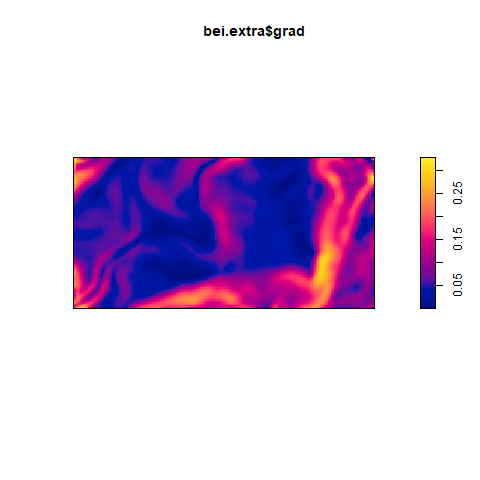
\includegraphics[width=6cm]{prob3_grad.png}
%     \caption{grad (for convenience to compare below plots)}
% \end{figure}
\begin{figure}[h]
    \centering
    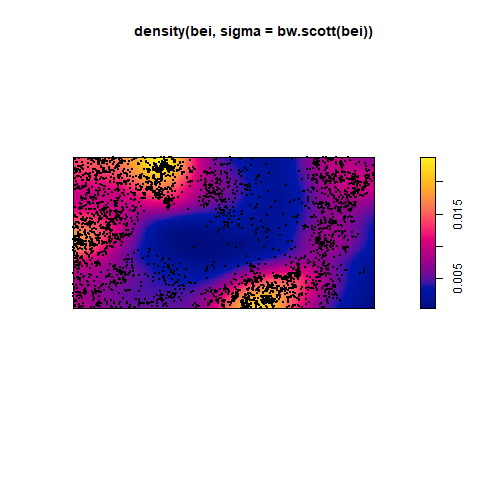
\includegraphics[width=6cm]{prob3_intensity_nocovariates.png} \\
    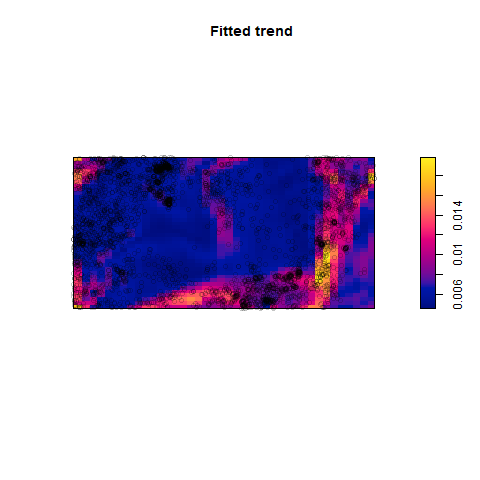
\includegraphics[width=6cm]{prob3_model1_fit.png}
    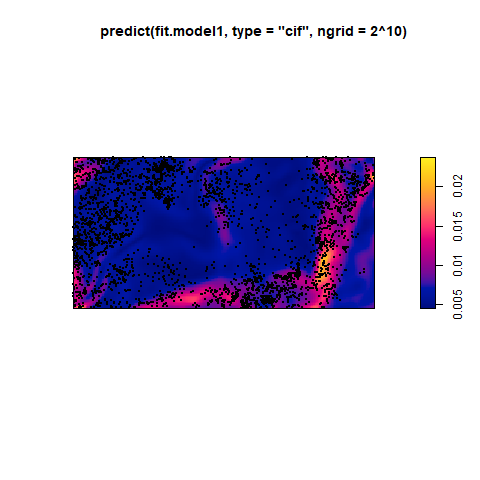
\includegraphics[width=6cm]{prob3_model1_predict.png} \\
    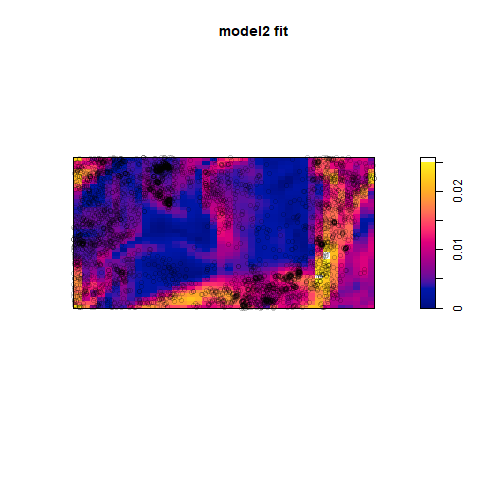
\includegraphics[width=6cm]{prob3_model2_fit.png}
    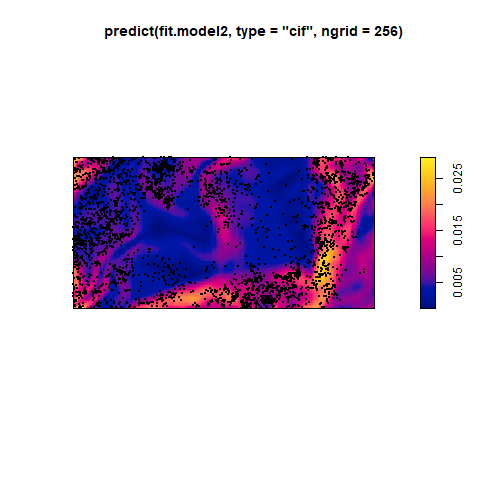
\includegraphics[width=6cm]{prob3_model2_predict.png}
    \caption{Estimated intensity functions: \\
    first row: no covariates\\
    second row: model 1 (left: fitted, right: predict(with more refined grid)) \\
    third row: model 2 (left: fitted, right: predict(with more refined grid))
    }
\end{figure}

\clearpage
Note that I use same scale for above five 2d-density plots.

When observing the plots, I can find that for model 1 and model 2,
the grad variable affects seriously to fitted results. 
Overall forms of model 1 and model 2 are similar to of grad so that the lower-right area has high intensity,
while the upper-left area has relatively lower, despite many points in there.
But it is natural result, because the models does not include other covariates like x-coordinate or y-coordinate,
but only grad variable. Thus the intensity cannot differ with form of grad.
If you compare these result to no covariate case (just gaussian kernel fit), this point is shown more remarkably.

Next, when we search for a difference between results of model 1 and of model 2,
we just find it in a view of overall level. It is because the model differs only on whether the model includes intercept or not.

\end{document}